\documentclass{article}

% content/resources/templates/preamble.tex
\usepackage[margin=0.6in]{geometry}
\author{Milav Dabgar}
\usepackage{amsmath,amssymb,amsthm}
\usepackage{booktabs}
\usepackage{multirow}
\usepackage{xcolor}
\usepackage{tcolorbox}
\tcbuselibrary{breakable,skins}
\usepackage[colorlinks=true,linkcolor=blue]{hyperref}
\usepackage{titlesec}
\usepackage{enumitem}
\usepackage{tikz}
\usepackage{pgfplots}
\usepackage{circuitikz}
\usepackage[version=4]{mhchem}
\usepackage{longtable}
\usepackage{array}
\usepackage{float}
\usepackage{caption}
\usepackage{listings}

\lstset{
  basicstyle=\small\ttfamily,
  breaklines=true,
  breakatwhitespace=false,
  postbreak=\mbox{\textcolor{red}{$\hookrightarrow$}\space},
  float=false,
  numbers=left,
  numberstyle=\tiny\color{gray},
  numbersep=10pt,
  xleftmargin=2em,
  keywordstyle=\color{blue},
  commentstyle=\color{green!60!black},
  stringstyle=\color{purple},
  backgroundcolor=\color{gray!5},
  showstringspaces=false,
  tabsize=2,
  captionpos=b,
  keepspaces=true,
  columns=flexible
}

\pgfplotsset{compat=1.18}
\usetikzlibrary{shapes,arrows,positioning,calc,patterns,decorations.pathmorphing,decorations.markings,arrows.meta}

% Color scheme
\definecolor{headcolor}{RGB}{0,102,204}
\definecolor{keycolor}{RGB}{220,20,60}
\definecolor{solutioncolor}{RGB}{34,139,34}
\definecolor{mnemoniccolor}{RGB}{148,0,211}
\definecolor{codecolor}{RGB}{0,0,100}

% Spacing
\setlength{\parskip}{3pt}
\setlist[itemize]{nosep}
\setlist[enumerate]{nosep}

% Title formatting
\titleformat{\section}{\Large\bfseries\color{headcolor}}{\thesection}{1em}{}
\titleformat{\subsection}{\large\bfseries\color{headcolor}}{\thesubsection}{1em}{}

% Pandoc tightlist compatibility
\providecommand{\tightlist}{%
  \setlength{\itemsep}{0pt}\setlength{\parskip}{0pt}}

% Pandoc longtable compatibility
\newcounter{none}
\def\thenone{}


% content/resources/templates/english-boxes.tex

% Custom environments
\newtcolorbox{solutionbox}{
 breakable,
 enhanced,
 colback=solutioncolor!5!white,
 colframe=solutioncolor!75!black,
 fonttitle=\bfseries,
 title=Solution
}

\newtcolorbox{solutionboxnobreak}{
 colback=solutioncolor!5!white,
 colframe=solutioncolor!75!black,
 fonttitle=\bfseries,
 title=Solution
}

\newtcolorbox{keyformula}{
 breakable,
 enhanced,
 colback=keycolor!5!white,
 colframe=keycolor!75!black,
 fonttitle=\bfseries,
 title=Key Formula
}

\newtcolorbox{mnemonicboxenv}{
 breakable,
 enhanced,
 colback=mnemoniccolor!5!white,
 colframe=mnemoniccolor!75!black,
 fonttitle=\bfseries,
 title=Mnemonic
}

\newcommand{\mnemonicbox}[1]{%
  \begin{mnemonicboxenv}
    #1
  \end{mnemonicboxenv}
}


% Custom commands for GTU solutions
% This file defines semantic commands for consistent formatting

% Question command with automatic formatting
\newcommand{\question}[2]{%
  \section*{Question #1}%
  \textbf{#2}%
}

% OR question variant
\newcommand{\questionor}[2]{%
  \section*{Question #1 OR}%
  \textbf{#2}%
}

% Proper table environment with caption
\newenvironment{answertable}[1]{%
  \begin{table}[htbp]
  \centering
  \caption{#1}
}{%
  \end{table}
}

% Proper figure environment for diagrams
\newenvironment{answerdiagram}[1]{%
  \begin{figure}[htbp]
  \centering
  \caption{#1}
}{%
  \end{figure}
}

% Semantic markup for key terms
\newcommand{\keyword}[1]{\textbf{#1}}
\newcommand{\code}[1]{\texttt{#1}}
\newcommand{\classname}[1]{\texttt{#1}}
\newcommand{\methodname}[1]{\texttt{#1}}

% Proper quotation marks
\newcommand{\mnemonic}[1]{``#1''}


\title{Data Structure with Python (4331601) - Winter 2023 Solution}
\date{January 11, 2024}

\begin{document}
\maketitle

\questionmarks{1(a)}{3}{Define best case, worst case and average case for time complexity.}

\begin{solutionbox}
\textbf{Answer}:

\begin{center}
\captionof{table}{Time Complexity Cases}
\begin{tabulary}{\linewidth}{|L|L|L|}
\hline
\textbf{Case Type} & \textbf{Definition} & \textbf{Example} \\
\hline
\textbf{Best Case} & Minimum time needed for algorithm execution & Linear search finds element at first position \\
\hline
\textbf{Worst Case} & Maximum time needed for algorithm execution & Linear search finds element at last position \\
\hline
\textbf{Average Case} & Expected time for typical input scenarios & Linear search finds element in middle \\
\hline
\end{tabulary}
\end{center}

\begin{itemize}
    \item \keyword{Best Case}: Algorithm performs optimally with ideal input conditions
    \item \keyword{Worst Case}: Algorithm takes maximum possible time with unfavorable input
    \item \keyword{Average Case}: Mathematical expectation of execution time across all possible inputs
\end{itemize}
\end{solutionbox}

\begin{mnemonicbox}
BWA - Best, Worst, Average
\end{mnemonicbox}

\questionmarks{1(b)}{4}{What is Class and Object in OOP? Give suitable example.}

\begin{solutionbox}
\textbf{Answer}:

\begin{center}
\captionof{table}{Class vs Object}
\begin{tabulary}{\linewidth}{|L|L|L|}
\hline
\textbf{Aspect} & \textbf{Class} & \textbf{Object} \\
\hline
\textbf{Definition} & Blueprint/template for creating objects & Instance of a class \\
\hline
\textbf{Memory} & No memory allocated & Memory allocated when created \\
\hline
\textbf{Example} & Car (template) & my\_car = Car() \\
\hline
\end{tabulary}
\end{center}

\begin{lstlisting}[language=Python,caption={Class and Object Example}]
# Class definition
class Student:
    def __init__(self, name, age):
        self.name = name
        self.age = age
    
    def display(self):
        print(f"Name: {self.name}, Age: {self.age}")

# Object creation
student1 = Student("John", 20)
student1.display()
\end{lstlisting}

\begin{itemize}
    \item \keyword{Class}: Template defining attributes and methods
    \item \keyword{Object}: Real instance with actual values
\end{itemize}
\end{solutionbox}

\begin{mnemonicbox}
Class = Cookie Cutter, Object = Actual Cookie
\end{mnemonicbox}

\questionmarks{1(c)}{7}{Write a program for two matrix multiplication using simple nested loop and numpy module.}

\begin{solutionbox}
\textbf{Answer}:

\begin{lstlisting}[language=Python,caption={Matrix Multiplication}]
# Method 1: Using Simple Nested Loop
def matrix_multiply_nested(A, B):
    rows_A, cols_A = len(A), len(A[0])
    rows_B, cols_B = len(B), len(B[0])
    
    # Initialize result matrix
    result = [[0 for _ in range(cols_B)] for _ in range(rows_A)]
    
    # Matrix multiplication
    for i in range(rows_A):
        for j in range(cols_B):
            for k in range(cols_A):
                result[i][j] += A[i][k] * B[k][j]
    
    return result

# Method 2: Using NumPy
import numpy as np

def matrix_multiply_numpy(A, B):
    A_np = np.array(A)
    B_np = np.array(B)
    return np.dot(A_np, B_np)

# Example usage
A = [[1, 2], [3, 4]]
B = [[5, 6], [7, 8]]

print("Nested Loop Result:", matrix_multiply_nested(A, B))
print("NumPy Result:", matrix_multiply_numpy(A, B))
\end{lstlisting}

\begin{itemize}
    \item \keyword{Nested Loop}: Three loops for row, column, and multiplication
    \item \keyword{NumPy}: Built-in dot() function for efficient multiplication
\end{itemize}
\end{solutionbox}

\begin{mnemonicbox}
Row $\times$ Column = Result
\end{mnemonicbox}

\questionmarks{1(c OR)}{7}{Write a program to implement basic operations on arrays.}

\begin{solutionbox}
\textbf{Answer}:

\begin{lstlisting}[language=Python,caption={Array Operations}]
import array

# Create array
arr = array.array('i', [1, 2, 3, 4, 5])

def array_operations():
    print("Original array:", arr)
    
    # Insert element
    arr.insert(2, 10)
    print("After insert(2, 10):", arr)
    
    # Append element
    arr.append(6)
    print("After append(6):", arr)
    
    # Remove element
    arr.remove(10)
    print("After remove(10):", arr)
    
    # Pop element
    popped = arr.pop()
    print(f"Popped element: {popped}, Array: {arr}")
    
    # Search element
    index = arr.index(3)
    print(f"Index of 3: {index}")
    
    # Count occurrences
    count = arr.count(2)
    print(f"Count of 2: {count}")

array_operations()
\end{lstlisting}

\begin{center}
\captionof{table}{Array Operations}
\begin{tabulary}{\linewidth}{|L|L|L|}
\hline
\textbf{Operation} & \textbf{Method} & \textbf{Description} \\
\hline
\textbf{Insert} & insert(index, value) & Add element at specific position \\
\hline
\textbf{Append} & append(value) & Add element at end \\
\hline
\textbf{Remove} & remove(value) & Remove first occurrence \\
\hline
\textbf{Pop} & pop() & Remove and return last element \\
\hline
\end{tabulary}
\end{center}
\end{solutionbox}

\begin{mnemonicbox}
IARP - Insert, Append, Remove, Pop
\end{mnemonicbox}

\questionmarks{2(a)}{3}{Explain Big 'O' Notation.}

\begin{solutionbox}
\textbf{Answer}:

\begin{center}
\captionof{table}{Big O Complexity}
\begin{tabulary}{\linewidth}{|L|L|L|}
\hline
\textbf{Notation} & \textbf{Name} & \textbf{Example} \\
\hline
\textbf{O(1)} & Constant & Array access \\
\hline
\textbf{O(n)} & Linear & Linear search \\
\hline
\textbf{O(n\textsuperscript{2})} & Quadratic & Bubble sort \\
\hline
\textbf{O(log n)} & Logarithmic & Binary search \\
\hline
\end{tabulary}
\end{center}

\begin{itemize}
    \item \keyword{Big O}: Describes upper bound of algorithm's time complexity
    \item \keyword{Purpose}: Compare efficiency of different algorithms
    \item \keyword{Focus}: Worst-case scenario analysis
\end{itemize}
\end{solutionbox}

\begin{mnemonicbox}
Big O = Big Order of growth
\end{mnemonicbox}

\questionmarks{2(b)}{4}{Differentiate between class method and static method.}

\begin{solutionbox}
\textbf{Answer}:

\begin{center}
\captionof{table}{Method Types Comparison}
\begin{tabulary}{\linewidth}{|L|L|L|}
\hline
\textbf{Aspect} & \textbf{Class Method} & \textbf{Static Method} \\
\hline
\textbf{Decorator} & @classmethod & @staticmethod \\
\hline
\textbf{First Parameter} & cls (class reference) & No special parameter \\
\hline
\textbf{Access} & Can access class variables & Cannot access class/instance variables \\
\hline
\textbf{Usage} & Alternative constructors & Utility functions \\
\hline
\end{tabulary}
\end{center}

\begin{lstlisting}[language=Python,caption={Class vs Static Method}]
class MyClass:
    class_var = "I am class variable"
    
    @classmethod
    def class_method(cls):
        return f"Class method accessing: {cls.class_var}"
    
    @staticmethod
    def static_method():
        return "Static method - no class access"

# Usage
print(MyClass.class_method())
print(MyClass.static_method())
\end{lstlisting}
\end{solutionbox}

\begin{mnemonicbox}
Class method has CLS, Static method is STandalone
\end{mnemonicbox}

\questionmarks{2(c)}{7}{Implement a class for single level inheritance using public and private type derivation.}

\begin{solutionbox}
\textbf{Answer}:

\begin{lstlisting}[language=Python,caption={Single Level Inheritance}]
# Base class
class Vehicle:
    def __init__(self, brand, model):
        self.brand = brand          # Public attribute
        self._model = model         # Protected attribute
        self.__year = 2023          # Private attribute
    
    def start_engine(self):
        return f"{self.brand} engine started"
    
    def _display_model(self):       # Protected method
        return f"Model: {self._model}"
    
    def __private_method(self):     # Private method
        return f"Year: {self.__year}"

# Derived class (Single level inheritance)
class Car(Vehicle):
    def __init__(self, brand, model, doors):
        super().__init__(brand, model)
        self.doors = doors
    
    def car_info(self):
        # Can access public and protected members
        return f"Car: {self.brand}, {self._display_model()}, Doors: {self.doors}"
    
    def demonstrate_access(self):
        print("Public access:", self.brand)
        print("Protected access:", self._model)
        # print("Private access:", self.__year)  # This would cause error

# Usage
my_car = Car("Toyota", "Camry", 4)
print(my_car.car_info())
print(my_car.start_engine())
my_car.demonstrate_access()
\end{lstlisting}

\begin{itemize}
    \item \keyword{Public}: Accessible everywhere (brand)
    \item \keyword{Protected}: Accessible in class and subclasses (\_model)
    \item \keyword{Private}: Only accessible within same class (\_\_year)
\end{itemize}
\end{solutionbox}

\begin{mnemonicbox}
Public = Everyone, Protected = Family, Private = Personal
\end{mnemonicbox}

\questionmarks{2(a OR)}{3}{Explain constructor with example.}

\begin{solutionbox}
\textbf{Answer}:

\begin{center}
\captionof{table}{Constructor Types}
\begin{tabulary}{\linewidth}{|L|L|L|}
\hline
\textbf{Type} & \textbf{Method} & \textbf{Purpose} \\
\hline
\textbf{Default} & \code{\_\_init\_\_(self)} & Initialize with default values \\
\hline
\textbf{Parameterized} & \code{\_\_init\_\_(self, params)} & Initialize with custom values \\
\hline
\end{tabulary}
\end{center}

\begin{lstlisting}[language=Python,caption={Constructor Example}]
class Student:
    def __init__(self, name="Unknown", age=18):  # Constructor
        self.name = name
        self.age = age
        print(f"Student {name} created")
    
    def display(self):
        print(f"Name: {self.name}, Age: {self.age}")

# Object creation calls constructor automatically
s1 = Student("Alice", 20)
s2 = Student()  # Uses default values
\end{lstlisting}

\begin{itemize}
    \item \keyword{Constructor}: Special method called when object is created
    \item \keyword{Purpose}: Initialize object attributes
    \item \keyword{Automatic}: Called automatically during object creation
\end{itemize}
\end{solutionbox}

\begin{mnemonicbox}
Constructor = Object's Birth Certificate
\end{mnemonicbox}

\questionmarks{2(b OR)}{4}{Write a program to demonstrate Polymorphism.}

\begin{solutionbox}
\textbf{Answer}:

\begin{lstlisting}[language=Python,caption={Polymorphism Example}]
# Base class
class Animal:
    def make_sound(self):
        pass

# Derived classes
class Dog(Animal):
    def make_sound(self):
        return "Woof!"

class Cat(Animal):
    def make_sound(self):
        return "Meow!"

class Cow(Animal):
    def make_sound(self):
        return "Moo!"

# Polymorphism demonstration
def animal_sound(animal):
    return animal.make_sound()

# Creating objects
animals = [Dog(), Cat(), Cow()]

# Same method call, different behavior
for animal in animals:
    print(f"{animal.__class__.__name__}: {animal_sound(animal)}")
\end{lstlisting}

\begin{center}
\captionof{table}{Polymorphism Benefits}
\begin{tabulary}{\linewidth}{|L|L|}
\hline
\textbf{Benefit} & \textbf{Description} \\
\hline
\textbf{Flexibility} & Same interface, different implementations \\
\hline
\textbf{Maintainability} & Easy to add new types \\
\hline
\textbf{Code Reuse} & Common interface for different objects \\
\hline
\end{tabulary}
\end{center}
\end{solutionbox}

\begin{mnemonicbox}
Poly = Many, Morph = Forms
\end{mnemonicbox}

\questionmarks{2(c OR)}{7}{Write a Python to implement multiple and hierarchical inheritance.}

\begin{solutionbox}
\textbf{Answer}:

\begin{lstlisting}[language=Python,caption={Inheritance Types}]
# Multiple Inheritance
class Teacher:
    def __init__(self, subject):
        self.subject = subject
    
    def teach(self):
        return f"Teaching {self.subject}"

class Researcher:
    def __init__(self, field):
        self.field = field
    
    def research(self):
        return f"Researching in {self.field}"

# Multiple inheritance
class Professor(Teacher, Researcher):
    def __init__(self, name, subject, field):
        self.name = name
        Teacher.__init__(self, subject)
        Researcher.__init__(self, field)
    
    def profile(self):
        return f"Prof. {self.name}: {self.teach()} and {self.research()}"

# Hierarchical Inheritance
class Vehicle:
    def __init__(self, brand):
        self.brand = brand
    
    def start(self):
        return f"{self.brand} started"

class Car(Vehicle):
    def drive(self):
        return f"{self.brand} car driving"

class Bike(Vehicle):
    def ride(self):
        return f"{self.brand} bike riding"

# Usage
prof = Professor("Smith", "Python", "AI")
print(prof.profile())

car = Car("Honda")
bike = Bike("Yamaha")
print(car.drive())
print(bike.ride())
\end{lstlisting}

\begin{center}
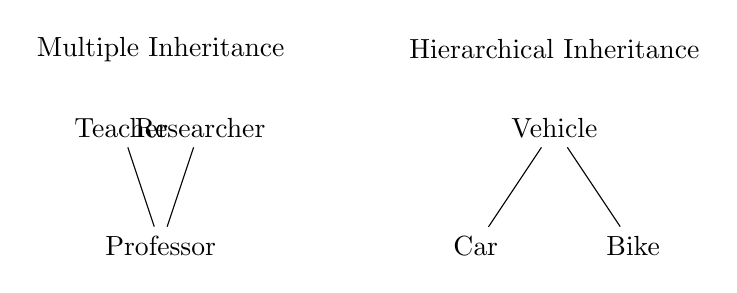
\begin{tikzpicture}[level 1/.style={sibling distance=2cm}, level 2/.style={sibling distance=1cm}]
    % Multiple Inheritance
    \node at (-3,0) {Multiple Inheritance};
    \node (T) at (-3.5,-1) {Teacher};
    \node (R) at (-2.5,-1) {Researcher};
    \node (P) at (-3,-2.5) {Professor};
    \draw (T) -- (P);
    \draw (R) -- (P);

    % Hierarchical Inheritance
    \node at (2,0) {Hierarchical Inheritance};
    \node (V) at (2,-1) {Vehicle};
    \node (C) at (1,-2.5) {Car};
    \node (B) at (3,-2.5) {Bike};
    \draw (V) -- (C);
    \draw (V) -- (B);
\end{tikzpicture}
\captionof{figure}{Inheritance Types}
\end{center}
\end{solutionbox}

\begin{mnemonicbox}
Multiple = Many Parents, Hierarchical = Tree Structure
\end{mnemonicbox}

\questionmarks{3(a)}{3}{Explain Push and Pop operations on Stack.}

\begin{solutionbox}
\textbf{Answer}:

\begin{center}
\captionof{table}{Stack Operations}
\begin{tabulary}{\linewidth}{|L|L|L|}
\hline
\textbf{Operation} & \textbf{Description} & \textbf{Time Complexity} \\
\hline
\textbf{Push} & Add element to top & O(1) \\
\hline
\textbf{Pop} & Remove element from top & O(1) \\
\hline
\textbf{Peek/Top} & View top element & O(1) \\
\hline
\textbf{isEmpty} & Check if stack is empty & O(1) \\
\hline
\end{tabulary}
\end{center}

\begin{lstlisting}[language=Python,caption={Stack Push-Pop}]
stack = []

# Push operation
stack.append(10)  # Push 10
stack.append(20)  # Push 20
print("After push:", stack)  # [10, 20]

# Pop operation
item = stack.pop()  # Pop 20
print(f"Popped: {item}, Stack: {stack}")  # [10]
\end{lstlisting}

\begin{itemize}
    \item \keyword{LIFO}: Last In, First Out principle
    \item \keyword{Top}: Only accessible element for operations
\end{itemize}
\end{solutionbox}

\begin{mnemonicbox}
Stack = Plate Stack - Last plate In, First plate Out
\end{mnemonicbox}

\questionmarks{3(b)}{4}{Explain Enqueue and Dequeue operations on Queue.}

\begin{solutionbox}
\textbf{Answer}:

\begin{center}
\captionof{table}{Queue Operations}
\begin{tabulary}{\linewidth}{|L|L|L|L|}
\hline
\textbf{Operation} & \textbf{Description} & \textbf{Position} & \textbf{Time Complexity} \\
\hline
\textbf{Enqueue} & Add element & Rear & O(1) \\
\hline
\textbf{Dequeue} & Remove element & Front & O(1) \\
\hline
\textbf{Front} & View front element & Front & O(1) \\
\hline
\textbf{Rear} & View rear element & Rear & O(1) \\
\hline
\end{tabulary}
\end{center}

\begin{lstlisting}[language=Python,caption={Queue Enqueue-Dequeue}]
from collections import deque

queue = deque()

# Enqueue operation
queue.append(10)  # Enqueue 10
queue.append(20)  # Enqueue 20
print("After enqueue:", list(queue))  # [10, 20]

# Dequeue operation
item = queue.popleft()  # Dequeue 10
print(f"Dequeued: {item}, Queue: {list(queue)}")  # [20]
\end{lstlisting}

\begin{itemize}
    \item \keyword{FIFO}: First In, First Out principle
    \item \keyword{Two ends}: Front for removal, Rear for insertion
\end{itemize}
\end{solutionbox}

\begin{mnemonicbox}
Queue = Line at Store - First person In, First person Out
\end{mnemonicbox}

\questionmarks{3(c)}{7}{Explain various applications of Stack.}

\begin{solutionbox}
\textbf{Answer}:

\begin{center}
\captionof{table}{Stack Applications}
\begin{tabulary}{\linewidth}{|L|L|L|}
\hline
\textbf{Application} & \textbf{Description} & \textbf{Example} \\
\hline
\textbf{Expression Evaluation} & Convert infix to postfix & (a+b)*c $\rightarrow$ ab+c* \\
\hline
\textbf{Function Calls} & Manage function call sequence & Recursion handling \\
\hline
\textbf{Undo Operations} & Reverse recent actions & Text editor undo \\
\hline
\textbf{Browser History} & Navigate back through pages & Back button \\
\hline
\textbf{Parentheses Matching} & Check balanced brackets & \{[()]\} validation \\
\hline
\end{tabulary}
\end{center}

\begin{lstlisting}[language=Python,caption={Parentheses Matching}]
# Example: Parentheses matching
def is_balanced(expression):
    stack = []
    pairs = {'(': ')', '[': ']', '{': '}'}
    
    for char in expression:
        if char in pairs:  # Opening bracket
            stack.append(char)
        elif char in pairs.values():  # Closing bracket
            if not stack:
                return False
            if pairs[stack.pop()] != char:
                return False
    
    return len(stack) == 0

# Test
print(is_balanced("({[]})"))  # True
print(is_balanced("({[}])"))  # False
\end{lstlisting}

\begin{itemize}
    \item \keyword{Memory Management}: Function call stack in programming
    \item \keyword{Backtracking}: Maze solving, game algorithms
    \item \keyword{Compiler Design}: Syntax analysis and parsing
\end{itemize}
\end{solutionbox}

\begin{mnemonicbox}
Stack Applications = UFPB (Undo, Function, Parentheses, Browser)
\end{mnemonicbox}

\questionmarks{3(a OR)}{3}{List out limitations of Single Queue.}

\begin{solutionbox}
\textbf{Answer}:

\begin{center}
\captionof{table}{Single Queue Limitations}
\begin{tabulary}{\linewidth}{|L|L|L|}
\hline
\textbf{Limitation} & \textbf{Description} & \textbf{Problem} \\
\hline
\textbf{Memory Wastage} & Front space becomes unusable & Inefficient memory usage \\
\hline
\textbf{Fixed Size} & Cannot resize dynamically & Space constraints \\
\hline
\textbf{False Overflow} & Queue appears full when front space empty & Premature capacity limit \\
\hline
\textbf{No Reuse} & Dequeued positions not reusable & Linear space utilization \\
\hline
\end{tabulary}
\end{center}

\begin{center}
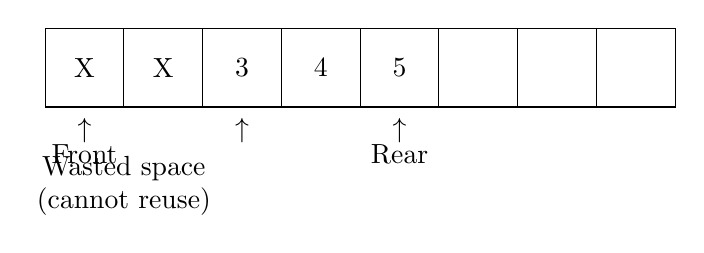
\begin{tikzpicture}
    \coordinate (A) at (0,0);
    \foreach \i/\val in {0/X, 1/X, 2/3, 3/4, 4/5, 5/, 6/, 7/} {
        \draw (\i,0) rectangle ++(1,1);
        \node at (\i+0.5, 0.5) {\val};
    }
    \node at (0.5, -0.3) {$\uparrow$};
    \node at (0.5, -0.6) {Front};
    \node at (2.5, -0.3) {$\uparrow$};
    \node at (4.5, -0.3) {$\uparrow$};
    \node at (4.5, -0.6) {Rear};
    
    \node[align=center] at (1, -1) {Wasted space\\(cannot reuse)};
\end{tikzpicture}
\captionof{figure}{Single Queue Problem}
\end{center}

\begin{itemize}
    \item \keyword{Linear Implementation}: Cannot utilize dequeued space
    \item \keyword{Static Array}: Fixed size allocation
\end{itemize}
\end{solutionbox}

\begin{mnemonicbox}
Single Queue = One-Way Street (No U-Turn)
\end{mnemonicbox}

\questionmarks{3(b OR)}{4}{Differentiate circular and simple queues.}

\begin{solutionbox}
\textbf{Answer}:

\begin{center}
\captionof{table}{Queue Types Comparison}
\begin{tabulary}{\linewidth}{|L|L|L|}
\hline
\textbf{Aspect} & \textbf{Simple Queue} & \textbf{Circular Queue} \\
\hline
\textbf{Memory Usage} & Linear, wasteful & Circular, efficient \\
\hline
\textbf{Space Reuse} & No reuse of dequeued space & Reuses all positions \\
\hline
\textbf{Overflow} & False overflow possible & True overflow only \\
\hline
\textbf{Implementation} & Front and rear pointers & Front and rear with modulo \\
\hline
\end{tabulary}
\end{center}

\begin{center}
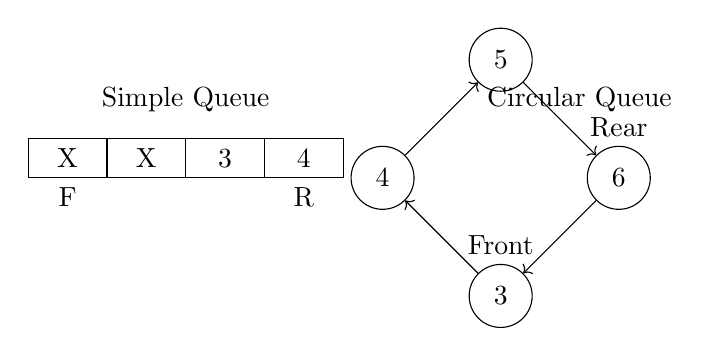
\begin{tikzpicture}
    % Simple Queue
    \node at (2, 2) {Simple Queue};
    \draw (0,1) rectangle (4,1.5);
    \foreach \x in {1,2,3} \draw (\x,1) -- (\x,1.5);
    \node at (0.5,1.25) {X}; \node at (1.5,1.25) {X};
    \node at (2.5,1.25) {3}; \node at (3.5,1.25) {4};
    \node[below] at (0.5,1) {F}; \node[below] at (3.5,1) {R};

    % Circular Queue
    \node at (7, 2) {Circular Queue};
    \foreach \i in {0,1,2,3} {
        \node[draw, circle, minimum size=0.8cm] (c\i) at ({6+1.5*cos(90-90*\i)}, {1+1.5*sin(90-90*\i)}) {};
    }
    \node at (c0) {5}; \node at (c1) {6}; \node at (c2) {3}; \node at (c3) {4};
    \draw[->] (c0) -- (c1); \draw[->] (c1) -- (c2); \draw[->] (c2) -- (c3); \draw[->] (c3) -- (c0);
    \node[above] at (c2.north) {Front};
    \node[above] at (c1.north) {Rear};
\end{tikzpicture}
\captionof{figure}{Simple vs Circular Queue}
\end{center}

\begin{lstlisting}[language=Python,caption={Circular Queue Implementation}]
class CircularQueue:
    def __init__(self, size):
        self.size = size
        self.queue = [None] * size
        self.front = -1
        self.rear = -1
    
    def enqueue(self, item):
        if (self.rear + 1) % self.size == self.front:
            print("Queue Full")
            return
        if self.front == -1:
            self.front = 0
        self.rear = (self.rear + 1) % self.size
        self.queue[self.rear] = item
    
    def dequeue(self):
        if self.front == -1:
            print("Queue Empty")
            return None
        item = self.queue[self.front]
        if self.front == self.rear:
            self.front = self.rear = -1
        else:
            self.front = (self.front + 1) % self.size
        return item
\end{lstlisting}
\end{solutionbox}

\begin{mnemonicbox}
Circular = Ring Road (Continuous), Simple = Dead End Street
\end{mnemonicbox}

\questionmarks{3(c OR)}{7}{Convert the following infix expression into postfix: (a * b) * (c \^{} (d + e) - f)}

\begin{solutionbox}
\textbf{Answer}:

\begin{center}
\captionof{table}{Operator Precedence}
\begin{tabulary}{\linewidth}{|L|L|L|}
\hline
\textbf{Operator} & \textbf{Precedence} & \textbf{Associativity} \\
\hline
\textbf{\^{}} & 3 & Right to Left \\
\hline
\textbf{*, /} & 2 & Left to Right \\
\hline
\textbf{+, -} & 1 & Left to Right \\
\hline
\end{tabulary}
\end{center}

\textbf{Step-by-step conversion:}

\begin{enumerate}
    \item (a * b) $\rightarrow$ ab*
    \item (d + e) $\rightarrow$ de+
    \item c \^{} (de+) $\rightarrow$ c de+ \^{}
    \item (c de+ \^{}) – f $\rightarrow$ c de+ \^{} f -
    \item (ab*) * (c de+ \^{} f -) $\rightarrow$ ab* c de+ \^{} f - *
\end{enumerate}

\textbf{Final Answer: ab*cde+\^{}f-*}

\begin{lstlisting}[language=Python,caption={Infix to Postfix}]
def infix_to_postfix(expression):
    precedence = {'+': 1, '-': 1, '*': 2, '/': 2, '^': 3}
    stack = []
    output = []
    
    for char in expression:
        if char.isalnum():
            output.append(char)
        elif char == '(':
            stack.append(char)
        elif char == ')':
            while stack and stack[-1] != '(':
                output.append(stack.pop())
            stack.pop()  # Remove '('
        elif char in precedence:
            while (stack and stack[-1] != '(' and 
                   stack[-1] in precedence and
                   precedence[stack[-1]] >= precedence[char]):
                output.append(stack.pop())
            stack.append(char)
    
    while stack:
        output.append(stack.pop())
    
    return ''.join(output)

# Test
result = infix_to_postfix("(a*b)*(c^(d+e)-f)")
print("Postfix:", result)  # ab*cde+^f-*
\end{lstlisting}
\end{solutionbox}

\begin{mnemonicbox}
PEMDAS for precedence, Stack for operators
\end{mnemonicbox}

\questionmarks{4(a)}{3}{List types of Linked List.}

\begin{solutionbox}
\textbf{Answer}:

\begin{center}
\captionof{table}{Linked List Types}
\begin{tabulary}{\linewidth}{|L|L|L|}
\hline
\textbf{Type} & \textbf{Description} & \textbf{Key Feature} \\
\hline
\textbf{Singly Linked} & One pointer to next node & Forward traversal only \\
\hline
\textbf{Doubly Linked} & Pointers to next and previous & Bidirectional traversal \\
\hline
\textbf{Circular Linked} & Last node points to first & No NULL pointer \\
\hline
\textbf{Doubly Circular} & Doubly + Circular features & Both directions + circular \\
\hline
\end{tabulary}
\end{center}

\begin{center}
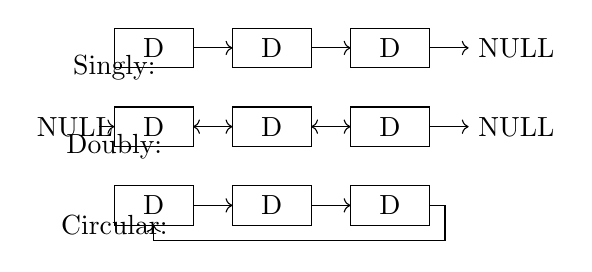
\begin{tikzpicture}
    % Singly
    \node at (0,3) {Singly:};
    \foreach \i in {0,1,2} \draw (\i*1.5, 3) rectangle ++(1,0.5) node[midway] {D};
    \draw[->] (1,3.25) -- (1.5,3.25); \draw[->] (2.5,3.25) -- (3,3.25); \draw[->] (4,3.25) -- (4.5,3.25) node[right] {NULL};
    
    % Doubly
    \node at (0,2) {Doubly:};
    \foreach \i in {0,1,2} \draw (\i*1.5, 2) rectangle ++(1,0.5) node[midway] {D};
    \draw[<->] (1,2.25) -- (1.5,2.25); \draw[<->] (2.5,2.25) -- (3,2.25);
    \node at (-0.5,2.25) {NULL}; \draw[<-] (0,2.25) -- (-0.2,2.25);
    \draw[->] (4,2.25) -- (4.5,2.25) node[right] {NULL};

    % Circular
    \node at (0,1) {Circular:};
    \foreach \i in {0,1,2} \draw (\i*1.5, 1) rectangle ++(1,0.5) node[midway] {D};
    \draw[->] (1,1.25) -- (1.5,1.25); \draw[->] (2.5,1.25) -- (3,1.25);
    \draw[->] (4,1.25) -- (4.2,1.25) -- (4.2,0.8) -- (0.5,0.8) -- (0.5,1);
\end{tikzpicture}
\captionof{figure}{Linked List Types}
\end{center}

\begin{itemize}
    \item \keyword{Memory}: Each node contains data and pointer(s)
    \item \keyword{Dynamic}: Size can change during runtime
\end{itemize}
\end{solutionbox}

\begin{mnemonicbox}
SDCD - Singly, Doubly, Circular, Doubly-Circular
\end{mnemonicbox}

\questionmarks{4(b)}{4}{Differentiate between circular linked list and singly linked list.}

\begin{solutionbox}
\textbf{Answer}:

\begin{center}
\captionof{table}{Singly vs Circular Linked List}
\begin{tabulary}{\linewidth}{|L|L|L|}
\hline
\textbf{Aspect} & \textbf{Singly Linked List} & \textbf{Circular Linked List} \\
\hline
\textbf{Last Node} & Points to NULL & Points to first node \\
\hline
\textbf{Traversal} & Ends at NULL & Continuous loop \\
\hline
\textbf{Memory} & Last node stores NULL & No NULL pointer \\
\hline
\textbf{Detection} & Check for NULL & Check for starting node \\
\hline
\end{tabulary}
\end{center}

\begin{lstlisting}[language=Python,caption={Singly vs Circular Traversal}]
# Singly Linked List Node
class SinglyNode:
    def __init__(self, data):
        self.data = data
        self.next = None

# Circular Linked List Node
class CircularNode:
    def __init__(self, data):
        self.data = data
        self.next = None

def traverse_singly(head):
    current = head
    while current:  # Stops at NULL
        print(current.data)
        current = current.next

def traverse_circular(head):
    if not head:
        return
    current = head
    while True:
        print(current.data)
        current = current.next
        if current == head:  # Back to start
            break
\end{lstlisting}
\end{solutionbox}

\begin{mnemonicbox}
Singly = Dead End, Circular = Race Track
\end{mnemonicbox}

\questionmarks{4(c)}{7}{Implement a program to perform following operation on singly linked list: a. Insert a node at the beginning of a singly linked list. b. Insert a node at the end of a singly linked list.}

\begin{solutionbox}
\textbf{Answer}:

\begin{lstlisting}[language=Python,caption={Singly Linked List Insertion}]
class Node:
    def __init__(self, data):
        self.data = data
        self.next = None

class SinglyLinkedList:
    def __init__(self):
        self.head = None
    
    def insert_at_beginning(self, data):
        """Insert node at the beginning"""
        new_node = Node(data)
        new_node.next = self.head
        self.head = new_node
        print(f"Inserted {data} at beginning")
    
    def insert_at_end(self, data):
        """Insert node at the end"""
        new_node = Node(data)
        
        if not self.head:  # Empty list
            self.head = new_node
            print(f"Inserted {data} at end (first node)")
            return
        
        # Traverse to last node
        current = self.head
        while current.next:
            current = current.next
        
        current.next = new_node
        print(f"Inserted {data} at end")
    
    def display(self):
        """Display the linked list"""
        if not self.head:
            print("List is empty")
            return
        
        current = self.head
        elements = []
        while current:
            elements.append(str(current.data))
            current = current.next
        
        print(" -> ".join(elements) + " -> NULL")

# Usage example
sll = SinglyLinkedList()

# Insert at beginning
sll.insert_at_beginning(10)
sll.insert_at_beginning(20)
sll.display()  # 20 -> 10 -> NULL

# Insert at end
sll.insert_at_end(30)
sll.insert_at_end(40)
sll.display()  # 20 -> 10 -> 30 -> 40 -> NULL
\end{lstlisting}

\begin{center}
\captionof{table}{Insertion Operations}
\begin{tabulary}{\linewidth}{|L|L|L|}
\hline
\textbf{Operation} & \textbf{Time Complexity} & \textbf{Steps} \\
\hline
\textbf{Beginning} & O(1) & 1. Create node 2. Point to head 3. Update head \\
\hline
\textbf{End} & O(n) & 1. Create node 2. Traverse to end 3. Link last node \\
\hline
\end{tabulary}
\end{center}
\end{solutionbox}

\begin{mnemonicbox}
Beginning = Quick (O(1)), End = Journey (O(n))
\end{mnemonicbox}

\questionmarks{4(a OR)}{3}{Explain doubly linked list.}

\begin{solutionbox}
\textbf{Answer}:

\begin{center}
\captionof{table}{Doubly Linked List Features}
\begin{tabulary}{\linewidth}{|L|L|}
\hline
\textbf{Feature} & \textbf{Description} \\
\hline
\textbf{Two Pointers} & prev and next in each node \\
\hline
\textbf{Bidirectional} & Can traverse forward and backward \\
\hline
\textbf{Memory} & Extra space for prev pointer \\
\hline
\textbf{Flexibility} & Easy insertion/deletion anywhere \\
\hline
\end{tabulary}
\end{center}

\begin{center}

\begin{tikzpicture}
    \node (null1) at (-1.5,0) {NULL};
    \foreach \i/\val in {0/A, 1/B, 2/C} {
        \draw (\i*2,0) rectangle ++(1.5,0.7) node[midway] {\val};
        \node[font=\tiny] at (\i*2+0.25, 0.15) {prev};
        \node[font=\tiny] at (\i*2+1.25, 0.15) {next};
    }
    \node (null2) at (6,0.35) {NULL};
    
    \draw[<-] (0,0.35) -- (null1);
    \draw[<->] (1.5,0.35) -- (2,0.35);
    \draw[<->] (3.5,0.35) -- (4,0.35);
    \draw[->] (5.5,0.35) -- (null2);
\end{tikzpicture}
\captionof{figure}{Doubly Linked List Structure}
\end{center}

\begin{itemize}
    \item \keyword{Advantages}: Bidirectional traversal, easier deletion
    \item \keyword{Disadvantages}: Extra memory for prev pointer
\end{itemize}
\end{solutionbox}

\begin{mnemonicbox}
Doubly = Two-Way Street
\end{mnemonicbox}

\questionmarks{4(b OR)}{4}{Describe applications of Linked List.}

\begin{solutionbox}
\textbf{Answer}:

\begin{center}
\captionof{table}{Linked List Applications}
\begin{tabulary}{\linewidth}{|L|L|L|}
\hline
\textbf{Application} & \textbf{Use Case} & \textbf{Benefit} \\
\hline
\textbf{Dynamic Arrays} & When size varies & Efficient memory usage \\
\hline
\textbf{Stack/Queue} & LIFO/FIFO operations & Dynamic size \\
\hline
\textbf{Graphs} & Adjacency list representation & Space efficient \\
\hline
\textbf{Music Playlist} & Previous/Next songs & Easy navigation \\
\hline
\textbf{Browser History} & Back/Forward navigation & Dynamic history \\
\hline
\textbf{Undo Operations} & Text editors & Efficient undo/redo \\
\hline
\end{tabulary}
\end{center}
\end{solutionbox}

\begin{mnemonicbox}
Linked Lists = Dynamic, Flexible, Connected
\end{mnemonicbox}

\questionmarks{4(c OR)}{7}{Implement Merge Sort algorithm.}

\begin{solutionbox}
\textbf{Answer}:

\begin{lstlisting}[language=Python,caption={Merge Sort Implementation}]
def merge_sort(arr):
    """Merge Sort implementation"""
    if len(arr) <= 1:
        return arr
    
    # Divide the array into two halves
    mid = len(arr) // 2
    left_half = arr[:mid]
    right_half = arr[mid:]
    
    # Recursively sort both halves
    left_sorted = merge_sort(left_half)
    right_sorted = merge_sort(right_half)
    
    # Merge the sorted halves
    return merge(left_sorted, right_sorted)

def merge(left, right):
    """Merge two sorted arrays"""
    result = []
    i = j = 0
    
    # Compare elements and merge
    while i < len(left) and j < len(right):
        if left[i] <= right[j]:
            result.append(left[i])
            i += 1
        else:
            result.append(right[j])
            j += 1
    
    # Add remaining elements
    result.extend(left[i:])
    result.extend(right[j:])
    
    return result

# Example usage
def demonstrate_merge_sort():
    arr = [64, 34, 25, 12, 22, 11, 90]
    print("Original array:", arr)
    
    sorted_arr = merge_sort(arr)
    print("Sorted array:", sorted_arr)

demonstrate_merge_sort()
\end{lstlisting}

\begin{center}
\captionof{table}{Merge Sort Analysis}
\begin{tabulary}{\linewidth}{|L|L|}
\hline
\textbf{Aspect} & \textbf{Value} \\
\hline
\textbf{Time Complexity} & O(n log n) \\
\hline
\textbf{Space Complexity} & O(n) \\
\hline
\textbf{Stability} & Stable \\
\hline
\textbf{Type} & Divide and Conquer \\
\hline
\end{tabulary}
\end{center}

\begin{itemize}
    \item \keyword{Divide}: Split array into two halves
    \item \keyword{Conquer}: Recursively sort both halves
    \item \keyword{Combine}: Merge sorted halves
\end{itemize}
\end{solutionbox}

\begin{mnemonicbox}
Merge Sort = Divide, Sort, Merge
\end{mnemonicbox}

\questionmarks{5(a)}{3}{Describe applications of binary tree.}

\begin{solutionbox}
\textbf{Answer}:

\begin{center}
\captionof{table}{Binary Tree Applications}
\begin{tabulary}{\linewidth}{|L|L|L|}
\hline
\textbf{Application} & \textbf{Description} & \textbf{Example} \\
\hline
\textbf{Expression Trees} & Mathematical expression representation & (a+b)*c \\
\hline
\textbf{Decision Trees} & Decision making in AI/ML & Classification algorithms \\
\hline
\textbf{File Systems} & Directory structure organization & Folder hierarchy \\
\hline
\textbf{Database Indexing} & B-trees for efficient searching & Database indices \\
\hline
\textbf{Huffman Coding} & Data compression technique & File compression \\
\hline
\textbf{Heap Operations} & Priority queues implementation & Task scheduling \\
\hline
\end{tabulary}
\end{center}

\begin{itemize}
    \item \keyword{Hierarchical Data}: Naturally represents tree-like structures
    \item \keyword{Efficient Search}: Binary search trees provide O(log n) operations
    \item \keyword{Memory Management}: Used in compiler design for syntax trees
\end{itemize}
\end{solutionbox}

\begin{mnemonicbox}
Binary Trees = EDFDHH (Expression, Decision, File, Database, Huffman, Heap)
\end{mnemonicbox}

\questionmarks{5(b)}{4}{Explain Indegree and Outdegree of Binary Tree with example.}

\begin{solutionbox}
\textbf{Answer}:

\begin{center}
\captionof{table}{Degree Definitions}
\begin{tabulary}{\linewidth}{|L|L|L|}
\hline
\textbf{Term} & \textbf{Definition} & \textbf{Binary Tree Value} \\
\hline
\textbf{Indegree} & Number of edges coming into a node & 0 (root) or 1 (others) \\
\hline
\textbf{Outdegree} & Number of edges going out of a node & 0, 1, or 2 \\
\hline
\textbf{Degree} & Total edges connected to node & Indegree + Outdegree \\
\hline
\end{tabulary}
\end{center}

\begin{center}
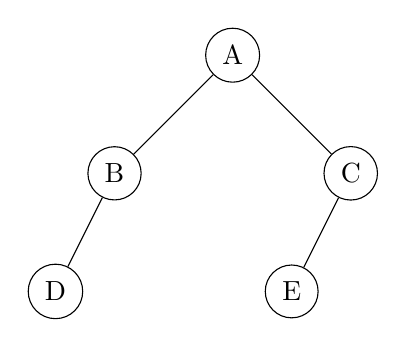
\begin{tikzpicture}[level 1/.style={sibling distance=3cm}, level 2/.style={sibling distance=1.5cm}]
    \node[circle, draw] {A}
        child {node[circle, draw] {B}
            child {node[circle, draw] {D}}
            child[missing]
        }
        child {node[circle, draw] {C}
            child {node[circle, draw] {E}}
            child[missing]
        };
\end{tikzpicture}
\captionof{figure}{Binary Tree Example}
\end{center}

\begin{center}
\captionof{table}{Example Analysis}
\begin{tabulary}{\linewidth}{|L|L|L|L|}
\hline
\textbf{Node} & \textbf{Indegree} & \textbf{Outdegree} & \textbf{Node Type} \\
\hline
A & 0 & 2 & Root \\
\hline
B & 1 & 1 & Internal \\
\hline
C & 1 & 1 & Internal \\
\hline
D & 1 & 0 & Leaf \\
\hline
E & 1 & 0 & Leaf \\
\hline
\end{tabulary}
\end{center}
\end{solutionbox}

\begin{mnemonicbox}
In = Coming In, Out = Going Out
\end{mnemonicbox}

\questionmarks{5(c)}{7}{Write a program to implement construction of binary search trees.}

\begin{solutionbox}
\textbf{Answer}:

\begin{lstlisting}[language=Python,caption={Binary Search Tree Construction}]
class TreeNode:
    def __init__(self, data):
        self.data = data
        self.left = None
        self.right = None

class BinarySearchTree:
    def __init__(self):
        self.root = None
    
    def insert(self, data):
        """Insert a node in BST"""
        if self.root is None:
            self.root = TreeNode(data)
        else:
            self._insert_recursive(self.root, data)
    
    def _insert_recursive(self, node, data):
        if data < node.data:
            if node.left is None:
                node.left = TreeNode(data)
            else:
                self._insert_recursive(node.left, data)
        elif data > node.data:
            if node.right is None:
                node.right = TreeNode(data)
            else:
                self._insert_recursive(node.right, data)
    
    def search(self, data):
        """Search for a node in BST"""
        return self._search_recursive(self.root, data)
    
    def _search_recursive(self, node, data):
        if node is None or node.data == data:
            return node
        
        if data < node.data:
            return self._search_recursive(node.left, data)
        else:
            return self._search_recursive(node.right, data)
    
    def inorder_traversal(self):
        """Inorder traversal (Left, Root, Right)"""
        result = []
        self._inorder_recursive(self.root, result)
        return result
    
    def _inorder_recursive(self, node, result):
        if node:
            self._inorder_recursive(node.left, result)
            result.append(node.data)
            self._inorder_recursive(node.right, result)

# Example usage
bst = BinarySearchTree()
values = [50, 30, 70, 20, 40, 60, 80]

print("Inserting values:", values)
for value in values:
    bst.insert(value)

print("\nInorder traversal:", bst.inorder_traversal())
\end{lstlisting}

\begin{center}
\captionof{table}{BST Operations}
\begin{tabulary}{\linewidth}{|L|L|L|}
\hline
\textbf{Operation} & \textbf{Time Complexity} & \textbf{Description} \\
\hline
\textbf{Insert} & O(log n) average, O(n) worst & Add new node \\
\hline
\textbf{Search} & O(log n) average, O(n) worst & Find specific node \\
\hline
\textbf{Delete} & O(log n) average, O(n) worst & Remove node \\
\hline
\textbf{Traversal} & O(n) & Visit all nodes \\
\hline
\end{tabulary}
\end{center}
\end{solutionbox}

\begin{mnemonicbox}
BST Rule = Left < Root < Right
\end{mnemonicbox}

\questionmarks{5(a OR)}{3}{Define level, degree and leaf node in binary tree.}

\begin{solutionbox}
\textbf{Answer}:

\begin{center}
\captionof{table}{Binary Tree Terms}
\begin{tabulary}{\linewidth}{|L|L|L|}
\hline
\textbf{Term} & \textbf{Definition} & \textbf{Example} \\
\hline
\textbf{Level} & Distance from root (root = level 0) & Root=0, Children=1, etc. \\
\hline
\textbf{Degree} & Number of children a node has & 0, 1, or 2 \\
\hline
\textbf{Leaf Node} & Node with no children (degree = 0) & Terminal nodes \\
\hline
\end{tabulary}
\end{center}

\begin{center}
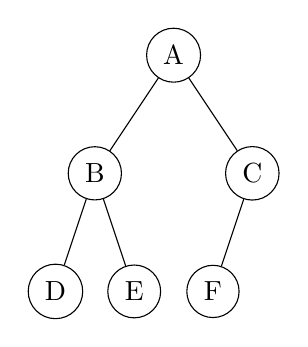
\begin{tikzpicture}[level 1/.style={sibling distance=2cm}, level 2/.style={sibling distance=1cm}]
    \node[circle, draw] {A}
        child {node[circle, draw] {B}
            child {node[circle, draw] {D}}
            child {node[circle, draw] {E}}
        }
        child {node[circle, draw] {C}
            child {node[circle, draw] {F}}
            child[missing]
        };
\end{tikzpicture}
\captionof{figure}{Binary Tree with Levels}
\end{center}

\begin{itemize}
    \item \keyword{Height}: Maximum level in tree
    \item \keyword{Depth}: Same as level for a node
\end{itemize}
\end{solutionbox}

\begin{mnemonicbox}
Level = Floor number, Degree = Children count, Leaf = No children
\end{mnemonicbox}

\questionmarks{5(b OR)}{4}{Explain complete binary tree with example.}

\begin{solutionbox}
\textbf{Answer}:

\begin{center}
\captionof{table}{Binary Tree Types}
\begin{tabulary}{\linewidth}{|L|L|L|}
\hline
\textbf{Type} & \textbf{Description} & \textbf{Property} \\
\hline
\textbf{Complete} & All levels filled except last, left-filled & Efficient array representation \\
\hline
\textbf{Full} & Every node has 0 or 2 children & No single-child nodes \\
\hline
\textbf{Perfect} & All levels completely filled & 2\textsuperscript{h} - 1 nodes \\
\hline
\end{tabulary}
\end{center}

\begin{center}
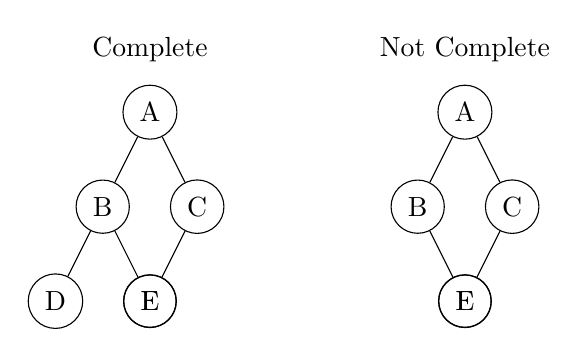
\begin{tikzpicture}[scale=0.8]
    \node at (0,3) {Complete};
    \node[circle,draw] at (0,2) {A}
        child {node[circle,draw] {B} child {node[circle,draw] {D}} child {node[circle,draw] {E}}}
        child {node[circle,draw] {C} child {node[circle,draw] {F}} child[missing]};

    \node at (5,3) {Not Complete};
    \node[circle,draw] at (5,2) {A}
        child {node[circle,draw] {B} child[missing] child {node[circle,draw] {E}}}
        child {node[circle,draw] {C} child {node[circle,draw] {F}} child[missing]};
\end{tikzpicture}
\captionof{figure}{Complete vs Non-Complete Binary Tree}
\end{center}

\begin{lstlisting}[language=Python,caption={Complete Binary Tree Structure}]
class CompleteBinaryTree:
    def __init__(self):
        self.tree = []
    
    def insert(self, data):
        """Insert in complete binary tree manner"""
        self.tree.append(data)
    
    def get_parent_index(self, i):
        return (i - 1) // 2
    
    def get_left_child_index(self, i):
        return 2 * i + 1
    
    def get_right_child_index(self, i):
        return 2 * i + 2
\end{lstlisting}
\end{solutionbox}

\begin{mnemonicbox}
Complete = All floors full except last, filled left to right
\end{mnemonicbox}

\questionmarks{5(c OR)}{7}{Construct a Binary Search Tree (BST) for the following sequence of numbers: 50, 70, 60, 20, 90, 10, 40, 100}

\begin{solutionbox}
\textbf{Answer}:

\textbf{Step-by-step BST Construction:}

\begin{enumerate}
    \item Insert 50: Root
    \item Insert 70: $70 > 50 \rightarrow$ Right
    \item Insert 60: $60 > 50 \rightarrow$ Right, $60 < 70 \rightarrow$ Left
    \item Insert 20: $20 < 50 \rightarrow$ Left
    \item Insert 90: $90 > 50 \rightarrow$ Right, $90 > 70 \rightarrow$ Right
    \item Insert 10: $10 < 50 \rightarrow$ Left, $10 < 20 \rightarrow$ Left
    \item Insert 40: $40 < 50 \rightarrow$ Left, $40 > 20 \rightarrow$ Right
    \item Insert 100: $100 > 50 \rightarrow$ Right... $100 > 90 \rightarrow$ Right
\end{enumerate}

\begin{center}
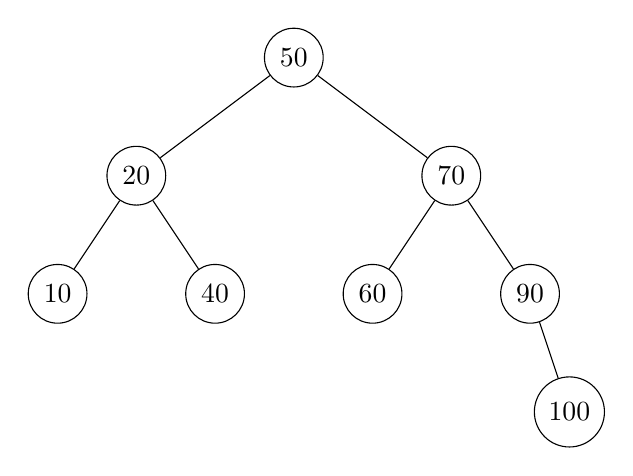
\begin{tikzpicture}[level 1/.style={sibling distance=4cm}, level 2/.style={sibling distance=2cm}, level 3/.style={sibling distance=1cm}]
    \node[circle, draw] {50}
        child {node[circle, draw] {20}
            child {node[circle, draw] {10}}
            child {node[circle, draw] {40}}
        }
        child {node[circle, draw] {70}
            child {node[circle, draw] {60}}
            child {node[circle, draw] {90}
                child[missing]
                child {node[circle, draw] {100}}
            }
        };
\end{tikzpicture}
\captionof{figure}{Final BST Structure}
\end{center}

\begin{lstlisting}[language=Python,caption={BST Construction}]
# Construct the BST
bst = BST()
sequence = [50, 70, 60, 20, 90, 10, 40, 100]

for num in sequence:
    bst.insert(num)
\end{lstlisting}

\begin{center}
\captionof{table}{Traversal Results}
\begin{tabulary}{\linewidth}{|L|L|}
\hline
\textbf{Traversal} & \textbf{Result} \\
\hline
\textbf{Inorder} & 10, 20, 40, 50, 60, 70, 90, 100 \\
\hline
\textbf{Preorder} & 50, 20, 10, 40, 70, 60, 90, 100 \\
\hline
\textbf{Postorder} & 10, 40, 20, 60, 100, 90, 70, 50 \\
\hline
\end{tabulary}
\end{center}
\end{solutionbox}

\begin{mnemonicbox}
BST Construction = Compare, Choose direction, Insert
\end{mnemonicbox}

\end{document}
